\notechapter{N-20251113}{When Addition Starts Floating: Theta-Links, Log-Links, and Arithmetic Deformation}

\section{What has to be explained}

The previous note ended with a deliberately strange operation.  At a bad split multiplicative valuation \(v\), one has a Tate parameter \(q_v\), and the arithmetic-deformation viewpoint takes seriously transformations of the shape
\[
  q_v\longmapsto q_v^{m^2},
  \qquad
  u\longmapsto u\quad (u\in\mathcal O_{F_v}^{\times}).
\]
This is not a ring homomorphism.  It is a transformation of multiplicative data.  The mathematical question is therefore precise:

\begin{center}
\emph{How can one deform multiplicative theta-data, lose ordinary additive compatibility, and still recover enough structure to prove an inequality?}
\end{center}

Fesenko's survey passes through nonarchimedean theta-functions, generalized Kummer theory, theta-links, log-links, log-shells, multiradial reconstruction, and indeterminacies.  Each object appears because the previous one no longer carries enough structure to compare the deformed multiplicative data.

\section{The nonarchimedean theta-function}

Let \(L\) be a local field of characteristic zero with finite residue field, and let \(C_L\) be the completion of an algebraic closure of \(L\).  Let \(q\in L\) be a nonzero element of the maximal ideal of \(\mathcal O_L\).  In the application to elliptic curves, \(q\) is the Tate parameter \(q_v\).

\begin{definition}[Theta-function of type \(a u^m\)]
A holomorphic function \(f:C_L^{\times}\to C_L\), defined over \(L\), is a theta-function of type \(a u^m\), where \(a\in C_L^{\times}\) and \(m\in\mathbb Z\), if
\[
  f(u)=a u^m f(qu).
\]
A meromorphic function invariant under \(u\mapsto qu\) descends to a function on the Tate quotient
\[
  C_L^{\times}/\langle q\rangle.
\]
\end{definition}

The basic nonarchimedean theta-function used in the survey is
\[
  \theta(u)=\sum_{n\in\mathbb Z}(-1)^n q^{n(n-1)/2}u^n.
\]
It also has the product expansion
\[
  \theta(u)=(1-u)\prod_{n\geq1}(1-q^n)(1-q^n u)(1-q^n u^{-1}),
\]
which is the nonarchimedean analogue of the Jacobi triple product expression.  The function is chosen because its zeros and poles interact well with the Tate curve and with the theta-values used in IUT.

\begin{remark}[Why a theta-function appears]
The theta-function is not added to the story for analogy with complex analysis alone.  On a Tate curve, elliptic functions with period \(q\) can be expressed in terms of theta-functions.  Thus theta-functions are a natural language for functions on the local analytic uniformization
\[
  E(L)\cong L^{\times}/\langle q\rangle.
\]
\end{remark}

Fesenko also records a modified theta-function, written here schematically as \(\ddot\Theta(u)\), whose special values at points separated by periods from \(\pm i\) satisfy a relation of the form
\[
  q^{m^2/2}\ddot\Theta\bigl(i\sqrt{q^m}\bigr)=\ddot\Theta(i).
\]
After choosing a \(2l\)-th root of \(q\), this leads to theta-values of the shape
\[
  \Theta\bigl(\sqrt{-q^m}\bigr)=q^{m^2},
  \qquad 1\leq m\leq \frac{l-1}{2},
\]
up to multiplication by roots of unity of order dividing \(2l\).

\begin{remark}[A controlled simplification]
The formula above is the correct structural feature needed here: special theta-values encode powers \(q^{m^2}\).  The complete IUT construction keeps track of coverings, labels, roots of unity, Galois actions, and compatible local-global data.  Those details are not being suppressed because they are unimportant; they are being postponed because the first conceptual step is to see why theta-values can serve as deformation data.
\end{remark}

\section{The local theta-link as a non-ring-theoretic map}

At a bad reduction valuation of odd residue characteristic, the main version of the theta-link described by Fesenko revolves around a local monoid-theoretic transformation.  In simplified notation it sends
\[
  q\longmapsto
  \bigl\{\Theta(\sqrt{-q^m})=q^{m^2}\bigr\}_{1\leq m\leq (l-1)/2},
\]
and it sends units to units by the identity map, up to the appropriate torsion ambiguity.

\begin{definition}[Local theta-link, structural form]
A local theta-link is a monoid-theoretic comparison which, at a bad split multiplicative valuation, keeps the unit part essentially fixed while replacing the Tate-period generator \(q\) by a family of theta-values behaving like \(q^{m^2}\).  It is a comparison of multiplicative and theta-theoretic data, not a homomorphism of local rings.
\end{definition}

Thus the local theta-link acts on two kinds of local data:
\[
  \mathcal O_L^{\times}/\operatorname{Tor}(\mathcal O_L^{\times}),
  \qquad
  \bigl\{q^{m^2}:1\leq m\leq (l-1)/2\bigr\},
\]
and it is glued to global monoid-theoretic data satisfying the product formula.

\begin{proposition}[Why the theta-link is not scheme-theoretic]
The theta-link is not compatible with the full ring structure of \(L\).  In particular, it should not be interpreted as a morphism of schemes or as a ring isomorphism between two local fields.
\end{proposition}

\begin{proof}
A ring homomorphism must preserve both multiplication and addition.  The theta-link is built from the multiplicative monoid of units, powers of the Tate parameter, and special values of a theta-function.  It transports multiplicative/theta data, but the additive operation of the local field is not transported by the displayed map.  Fesenko therefore describes this as an arithmetic deformation of the local structure rather than as an ordinary scheme-theoretic morphism.
\end{proof}

This is the first honest meaning of the phrase ``addition starts floating''.  It does not mean that the equation \(1+1=2\) becomes false inside a fixed field.  It means that after theta-deformation one is no longer allowed to identify the additive coordinates on the two sides as if a ring homomorphism had carried them across.

\section{The bridge supplied by Kummer theory}

If the theta-link only destroyed additive compatibility, it would not be useful.  The next ingredient explains how monoid-theoretic data can still communicate with Galois and fundamental-group data.

\begin{definition}[Kummer map, schematic form]
Let \(H\) be an open subgroup of a Galois or arithmetic fundamental group acting on an abelian group \(M\).  Kummer theory studies maps of the form
\[
  M^H\longrightarrow H^1\bigl(H,\operatorname{Hom}(\mathbb Q/\mathbb Z,M)\bigr),
\]
obtained by considering divisibility of elements of \(M\).
\end{definition}

For ordinary intuition, Kummer theory turns the question of extracting roots into a cohomological Galois datum.  In IUT, the relevant versions are generalized and truncated.  They are applied not merely to elements of fields, but also to monoid-theoretic structures associated with theta-functions, theta-values, number fields, and their completions.

\begin{remark}[Kummer theory as a translator]
The theta-link is monoid-theoretic.  Mono-anabelian reconstruction works on the side of arithmetic fundamental groups.  Kummer theory is one of the translators between these languages.  It relates theta-values and monoid data to Galois or fundamental-group structures that can be reconstructed and compared.
\end{remark}

A key issue here is cyclotomic rigidity.  Various copies of \(\widehat{\mathbb Z}\), or quotients of such copies, arise from roots of unity, from monoid-theoretic data, and from subquotients of fundamental groups.  IUT needs algorithms that identify the relevant cyclotomic structures in a canonical way.  Without such rigidity, the roots of unity introduced by extracting \(l\)-th or \(2l\)-th roots would create uncontrolled ambiguity.

\section{Two symmetries and the bookkeeping of labels}

The theta-link is built after choosing a prime \(l>3\).  The \(l\)-torsion points of the elliptic curve provide labels modeled on \(\mathbb F_l\).  Fesenko emphasizes two different symmetries.

\begin{definition}[The two label symmetries]
The geometric-additive symmetry is
\[
  \mathbb F_l^{\rtimes\pm}=\mathbb F_l\rtimes\{\pm1\},
\]
acting on labels by
\[
  z\longmapsto \pm z+a.
\]
The arithmetic-multiplicative symmetry is
\[
  \mathbb F_l^{\ast\pm}=\mathbb F_l^{\times}/\{\pm1\}.
\]
\end{definition}

The first symmetry is essentially geometric.  It is related to the geometric part of the arithmetic fundamental groups and to Kummer theory around theta-values.  It is also used to synchronize conjugacy ambiguities of local Galois groups attached to different labels.

The second symmetry is essentially arithmetic.  It is related to the Galois action of number fields and is multiplicative by definition.  It helps separate the zero label from the nonzero labels and is more naturally multiradial.

\begin{center}
\begin{tabular}{c|c|c}
\toprule
Symmetry & Nature & Role \\
\midrule
\(\mathbb F_l^{\rtimes\pm}\) & geometric/additive & conjugate synchronization \\
\(\mathbb F_l^{\ast\pm}\) & arithmetic/multiplicative & label bookkeeping and descent \\
\bottomrule
\end{tabular}
\end{center}

\begin{remark}[Why labels are not cosmetic]
The labels are not merely indices in a long construction.  They keep track of different copies of local Galois data and theta-values.  If these labels are identified too naively, one loses the distinction between the geometric-additive and arithmetic-multiplicative parts of the construction.
\end{remark}

\section{Conjugate synchronization and the basepoint problem}

Fundamental groups depend on basepoints.  In ordinary expositions this dependence is often hidden because different basepoints lead to groups identified up to inner automorphism.  In IUT this ambiguity cannot simply be ignored, because the theta-link and log-link compare structures that live in different theaters.

\begin{definition}[Conjugate synchronization, informal]
Conjugate synchronization is a system of identifications between local absolute Galois groups attached to different labels, arranged so that one does not introduce uncontrolled conjugacy indeterminacy.
\end{definition}

The need for such synchronization is one reason the theory becomes much more rigid than a naive ``copy-and-paste'' of local fields.  The comparison is not allowed to choose arbitrary basepoint identifications.  It must respect the label symmetries and the Kummer-theoretic data surrounding the theta-values.

\section{The log-link: recovering additive structure from multiplicative structure}

The theta-link uses multiplicative theta-values.  To regain access to additive structure, Fesenko turns to the nonarchimedean logarithm.

\begin{definition}[Nonarchimedean logarithm]
For a local field \(L\), the nonarchimedean logarithm
\[
  \log:\mathcal O_L^{\times}\longrightarrow L
\]
is defined on elements \(1-\alpha\), with \(\alpha\) in the maximal ideal of \(\mathcal O_L\), by
\[
  \log(1-\alpha)=-\sum_{n\geq1}\frac{\alpha^n}{n},
\]
and sends multiplicative representatives of the finite residue field to \(0\).
\end{definition}

The key point is that \(\log\) transforms multiplication into addition where it is defined.  Thus the logarithm lets multiplicative unit data speak an additive language.

\begin{definition}[Log-link, structural form]
A log-link is the comparison which shifts multiplicative unit data through the nonarchimedean logarithm, so that additive structures can be reconstructed from logarithmic images of multiplicative structures.
\end{definition}

Fesenko explains the relation between the two links as follows.  The multiplicative structures on the two sides of the theta-link are related through value-group data.  The additive structures are related through unit-group data after applying the log-link.

\begin{remark}[Why the logarithm is not optional]
Theta-values naturally act on multiplicative data, not directly on the additive group of the local field.  The logarithm creates a setting where multiplicative unit data has an additive image.  This is why the log-link is not an auxiliary simplification; it is part of the reconstruction mechanism.
\end{remark}

\section{The log-theta-lattice}

The theta-link and log-link do not appear as isolated arrows.  They are organized into a two-dimensional pattern called the log-theta-lattice.

\begin{definition}[Log-theta-lattice, schematic]
The log-theta-lattice is a two-dimensional array of theaters.  Vertical arrows are log-links, and horizontal arrows are theta-links.  A horizontal theta-link at one level depends on the log-link structure immediately below it.
\end{definition}

The picture is:

\begin{center}
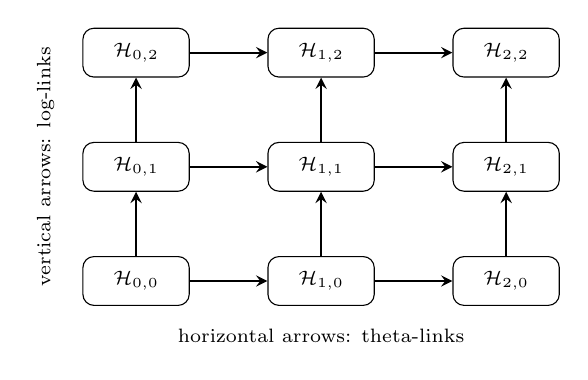
\begin{tikzpicture}[
  >=stealth,
  theater/.style={draw,rounded corners,minimum width=1.35cm,minimum height=0.62cm,align=center,font=\scriptsize},
  link/.style={->,thick}
]
  \node[theater] (H00) at (0,0) {\(\mathcal H_{0,0}\)};
  \node[theater] (H10) at (2.35,0) {\(\mathcal H_{1,0}\)};
  \node[theater] (H20) at (4.70,0) {\(\mathcal H_{2,0}\)};
  \node[theater] (H01) at (0,1.45) {\(\mathcal H_{0,1}\)};
  \node[theater] (H11) at (2.35,1.45) {\(\mathcal H_{1,1}\)};
  \node[theater] (H21) at (4.70,1.45) {\(\mathcal H_{2,1}\)};
  \node[theater] (H02) at (0,2.90) {\(\mathcal H_{0,2}\)};
  \node[theater] (H12) at (2.35,2.90) {\(\mathcal H_{1,2}\)};
  \node[theater] (H22) at (4.70,2.90) {\(\mathcal H_{2,2}\)};

  \foreach \j in {0,1,2} {
    \draw[link] (H0\j) -- (H1\j);
    \draw[link] (H1\j) -- (H2\j);
  }
  \foreach \i in {0,1,2} {
    \draw[link] (H\i0) -- (H\i1);
    \draw[link] (H\i1) -- (H\i2);
  }

  \node[font=\scriptsize,align=center] at (2.35,-0.70) {horizontal arrows: theta-links};
  \node[font=\scriptsize,align=center,rotate=90] at (-1.15,1.45) {vertical arrows: log-links};
\end{tikzpicture}
\end{center}

This diagram is only a guide.  Fesenko notes that the main results use just two neighboring infinite vertical lines and the horizontal arrow between the lattice points \((0,0)\) and \((1,0)\).  The important idea is that the theory does not compare a single source and target once.  It studies a controlled pattern of comparisons.

\section{The log-shell: a common container for incompatible links}

A technical difficulty now appears.  The log-link does not commute with the theta-link.  If one expected a clean commutative square, one would be disappointed.  IUT instead introduces a common structure that can hold the relevant images even when elementwise compatibility fails.

\begin{definition}[Log-shell]
For a nonarchimedean local field \(L\), the nonarchimedean part of the log-shell is a compact subgroup of the form
\[
  (p^{\ast})^{-1}\log(\mathcal O_L^{\times}),
\]
where \(p^{\ast}=p\) if \(p\) is odd and \(2^{\ast}=4\).  At a complex archimedean place, the corresponding log-shell is the closed ball of radius \(\pi\).
\end{definition}

The log-shell should not be imagined as an error bar in a numerical approximation.  It is a structural container.  The relevant Kummer isomorphisms are not compatible with the log-link at the level of individual elements, but their images are contained in the log-shell.  This is exactly the kind of weakened compatibility that arithmetic deformation needs.

\begin{remark}[Compatibility without equality]
In ordinary algebra one often tries to prove that a diagram commutes element by element.  The log-shell records a weaker but controlled form of compatibility: one compares inclusions of certain subsets or regions rather than exact equality of individual transported elements.
\end{remark}

\section{Mono-anabelian reconstruction and multiradiality}

The words ``reconstruction'' and ``multiradiality'' are easy to mystify, but their roles are concrete.

\begin{definition}[Mono-anabelian reconstruction]
Mono-anabelian reconstruction is the construction of ring-theoretic data from a single topological group that is known to be isomorphic to an arithmetic fundamental group of a suitable hyperbolic curve or orbicurve.  The reconstruction is algorithmic and functorial in the sense needed for localization and change of base field.
\end{definition}

The difference from ordinary anabelian comparison is important.  Classical anabelian geometry often compares two geometric objects through an isomorphism of their fundamental groups.  Mono-anabelian geometry asks for algorithms that start from one suitable group and recover the ring structure associated to it.

\begin{definition}[Multiradial algorithm]
A reconstruction algorithm is multiradial if an object constructed from one spoke of a wheel-like system is described in terms that still make sense from the viewpoint of other spokes.  Equivalently, it is compatible with simultaneous execution at multiple spokes.
\end{definition}

Here the ``wheel and spokes'' language is only an analogy, but a useful one.  A spoke corresponds to one theater or one radial perspective.  The center corresponds to a core object reconstructed from data that can be described from more than one spoke.

\begin{center}
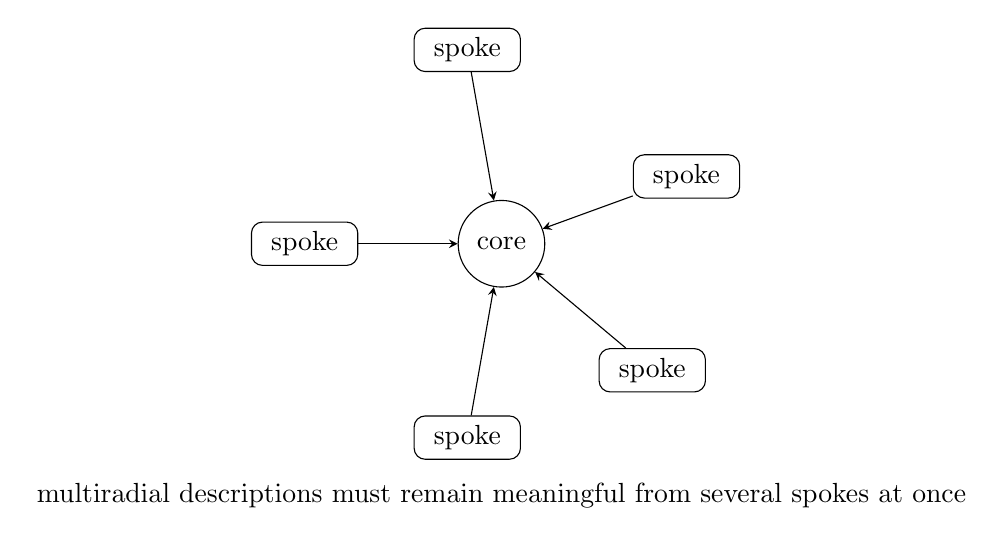
\begin{tikzpicture}[scale=1.0,>=stealth]
  \node[draw,circle,minimum size=1.1cm] at (0,0) (C) {core};
  \foreach \ang/\lab in {20/{spoke},100/{spoke},180/{spoke},260/{spoke},320/{spoke}} {
    \node[draw,rounded corners,minimum width=1.35cm,minimum height=0.55cm] at (\ang:2.5) (S\ang) {\lab};
    \draw[->] (S\ang) -- (C);
  }
  \node[align=center] at (0,-3.2) {multiradial descriptions must remain meaningful\ from several spokes at once};
\end{tikzpicture}
\end{center}

\begin{remark}[Why indeterminacy appears]
A multiradial description is stronger than a one-spoke description.  To make such descriptions possible, IUT allows certain controlled indeterminacies.  These are not defects added after the fact; they are part of how the theory avoids making illegal identifications between different theaters.
\end{remark}

\section{The three indeterminacies}

Fesenko singles out three indeterminacies that enter the computation of volume deformation.

\begin{definition}[The three indeterminacies, structural form]
The three main indeterminacies are:
\begin{enumerate}
  \item \(\mathrm{Ind1}\): an indeterminacy related to permutation symmetries of Galois and arithmetic fundamental groups along vertical lines of the log-theta-lattice;
  \item \(\mathrm{Ind2}\): an indeterminacy related to the horizontal theta-link and to the action of a compact group on \(\log(\mathcal O_L^{\times})\);
  \item \(\mathrm{Ind3}\): an indeterminacy arising from upper semi-compatibility of Kummer isomorphisms with log-links in a single vertical line.
\end{enumerate}
\end{definition}

The third phrase, ``upper semi-compatibility'', is deliberately weaker than commutativity of a diagram.  Instead of asking for equality of transported elements, one asks for controlled inclusion relations among the relevant subsets.

\begin{proposition}[Why indeterminacies are mathematically productive]
The indeterminacies do not merely obscure the comparison.  They make it possible to compare data across distinct theaters without falsely identifying the full ring structures on the two sides.
\end{proposition}

\begin{proof}
The theta-link is not ring-theoretic, and the log-link does not commute with it.  Therefore an elementwise comparison of ordinary rings would impose more structure than the construction provides.  The indeterminacies specify exactly which ambiguity is allowed: permutation ambiguity, horizontal theta-link ambiguity, and weakened Kummer/log compatibility.  A volume computation can then be performed after enlarging the target by these controlled ambiguities.
\end{proof}

This is where the intuitive phrase ``floating addition'' becomes mathematically safer.  The additive structure is not discarded into chaos.  It is reconstructed through logarithmic images and fundamental-group algorithms, while the unavoidable ambiguity is measured by the three indeterminacies.

\section{What the second note adds}

We can now summarize the actual mechanism more accurately than by saying ``IUT uses many universes''.

\begin{enumerate}
  \item The Tate parameter \(q\) gives local multiplicative data at bad reduction valuations.
  \item Nonarchimedean theta-functions produce distinguished values behaving like \(q^{m^2}\).
  \item The theta-link transports this theta/multiplicative data but is not a ring morphism.
  \item Generalized Kummer theory relates monoid-theoretic data to Galois and arithmetic fundamental-group data.
  \item The two label symmetries separate the geometric-additive side from the arithmetic-multiplicative side.
  \item The log-link uses \(\log:\mathcal O_L^{\times}\to L\) to recover additive information from multiplicative units.
  \item The log-shell supplies a common container when the log-link and theta-link fail to commute elementwise.
  \item Mono-anabelian reconstruction and multiradial algorithms make it possible to describe reconstructed objects from several theaters at once.
  \item The three indeterminacies specify the allowed ambiguity and enter the final volume estimate.
\end{enumerate}

The next note should therefore not treat the controversy around IUT as a piece of mathematical news.  The foundational issue is already visible here: once ordinary ring-theoretic identification is forbidden, the theory must replace it by theta-links, log-links, Kummer correspondences, and multiradial reconstruction.  The controversy is ultimately about whether this replacement is strong enough, not about whether the vocabulary is unusual.
